\documentclass{report}
\usepackage[utf8]{inputenc}
\usepackage{graphicx}
\usepackage{amssymb}
\usepackage{amsmath}
\usepackage{gensymb}
\usepackage{hyperref}
\usepackage{amsfonts}
\usepackage{biblatex} 

\title{Study of liquid brines on martial slopes}
\author{Khalid Koumila}
\date{}
\addbibresource{sample.bib} %Imports bibliography file

\begin{document}

\maketitle
\tableofcontents 

\newpage
\section*{Introduction}
The subject of water on Mars is controversial and remains a primary subject for the studies on the planet. 

Whereas there are proofs of ancient water present on Mars, whether it be by orbital observation or direct Rover exploration, little is known about present-day hydrology or lack thereof. 

Understanding the processes that drive the climate of Mars is necessary to understand our own climatology, as well as potential prospects for life.

Remote observations are the primary source of the processes that occur on the surface of the planet, and gives us insights on what is the structure and evolution of the interior.

In order for these observations to be interpreted, a certain theoretical work is needed to discriminate between competing theories that explain the same phenomenon.
In particular, recurring slope lineae are dark streaks recently observed by Mars Reconnaissance Orbiter (MRO) on the slopes of Mars. Their characteristics (location and orientation, seasonality) are compelling in the sense that they point to a liquid triggered event. 

In this work a model of temperature evolution will be set up in order to determine the possibility of the melting of subsurface ice. The investigation relies on the thermal study on the slope, taking into account the angle of the Sun and relevant variables.

\chapter{Background}
To understand the context in which this question arises, an overview of the current knowledge and exploration of Mars is given here.
\section{Exploration of Mars.} 
The planet is known since the antiquity, and subsequent observations yielded the existence of \textit{canali}, from Giovanni Schiaparelli, and subsequent theories about their artificial origins.

The distance to the Earth and poor quality of the instruments didn't allow a real investigation of present-day processes on Mars before the first orbiters and landers. The Soviet Marsnik and American Mariner spacecrafts were launched in the 1960's, with the first successes being Mariner 4 and Marsnik 5 in 1965 and 1974 respectively. 
The Vikings landers gave one of the first images from the surface of Mars from 1975 until the 1980's.

Mars Global Surveyor, launched in 1996, marked a new beginning in the exploration of Mars, closely followed by the rover Pathfinder and Mars Odyssey in 2001.
The orbiter that interests us is Mars Reconnaissance Orbiter, equipped with a high-resolution camera, HiRISE, that have a resolution of the order of 30 cm/pixel. 
This is the highest resolution yet achieved, and was instrumental in detecting and observing recurring slope lineae.

Improved technology and sensors are shipped with each generation of spacecrafts, the most recent being the lander InSight.

\section{Marian geology and climate}
Observation of the surface may be done by orbiting spacecrafts. The landforms observed indicate the processes that occurred on the planet at earlier times. The signs attest of the rich past of the interior, including volcanism, magnetic fields, tectonism and glaciers.

The primary feature of the surface of the planet is the hemispheric dichotomy. 
The Northern Hemisphere has a lower elevation and smoother surface than the Southern Hemisphere, which is older and show signs of craterization dating to the Late Heavy Bombardment.

Signs of ancient water presence are shown in erosion patterns, including the Valles Marineris, outflow channels and chaotic terrains. The presence of hydrated minerals is also documented by spectrometry and direct observation. 

Present water occurrence on Mars is limited to drops at the location of Phoenix lander.

Despite having a tenuous atmosphere (600 Pa) and no current magnetic field, Mars has a climate, in the sense of a general circulation, polar ice caps, and weather patterns due to the seasons. 
The eccentricity of Mars (0.0934) is greater than the Earth's (0.016), that has big impact on the duration of seasons and variations on solar insolation. 

\section{Description of the phenomena, characteristics, features.}
The observation of Recurring Slope Lineae (or RSL) follows certain patterns that are detailed in this section.

They are observed in the intermediate southern latitudes - around 40 \degree of latitude on slopes greater than 30 \degree, as well as near the equator (RSL candidates at Gale crater). 

Their presence is documented quasi exclusively on equator-facing slopes, sometimes west- or east- facing slopes, and exceptionally on polar facing slopes (as in Horowitz Crater, -32 \degree south). The south hemisphere being heavily craterized, one can expect the existence of slopes of all azimuths being represented. This piece of information points to a seminal role of the sun and direct solar rays input. 

The surface darkening is the first marker of the event, extending downslope. The origin of the albedo change is thought to be due to a rearrangement of the soil grains, after mixing with salty water or granular flow.  

Their lengths is of tens of meters with only tens of centimetres in width. They can only be resolved by high-resolution imaging systems such as HiRISE. 

They exhibit a seasonality, being only formed during local spring or summer, and vanishing towards the winter.
The orientation of the portion of the slope in which they occur is also determined to be preferentially toward the equator. 
The advance of the flow has higher rates at the beginning of the season.

\section{Previous works}

Since their first observations in 2008, many works were done investigating the origin of Recurring Slope Lineae.
We find traces of perchlorate at Pheonix landing site and remote sensing evidence of their presence on the site of known RSL, E. K. Leask et al. (2018) pointed a glitch in the post-acquisition treatment that resulted in artefacts that mimics the signature of various salts including perchlorates. Some Perchlorate reported location cannot be considered robust observations.  
If Chevrier (2012) investigates the temperature necessary for a melting of brines, based on a subsurface ice model adapted from Aharonson (2006), there have been critics of the liquid flow, e.g. McEwen (2018) that is a proponent of the granular flow theory. Stillman (2018) distinguish the cases of wet-dominated flow, wet-triggered flow and dry granular flow, concluding that no mechanism can be the sole origin of the process. 
As for near-equator RSLs, that have different characteristics, Stillman (2016) suggests a strong link with a briny aquifer upwelling.  

All papers concur that new data and enhanced models must be combined to describe accurately the observations. 

\chapter{Model}
The model used is a combination of a 1-D thermal model for planetary surface, and various hypothesis done about the composition and structure of the soil, based on available information, observation and study of martian soil analogues. 

\section{1-D thermal model}
The source code is adapted from the work of Schorghofer (2015), written in fortran language. 
It describes the energy balance equation for the surface, as the following :
\[\rho c \frac{dT}{dt}=k\frac{d^2 T}{dz^2}\]

    \subsection{Boundary conditions}
It is solved with a semi-implicit Crank-Nicholson scheme with the addition of the upper boundary condition: 
\[Q + k \frac{dT}{dz} = \epsilon \sigma T^4\] 

The Q is itself a combination of direct sunlight input, scattered solar rays in the atmosphere coming from the whole half-sphere, and contribution due to IR emission of the atmospheres. These as defined with the help of the solar zenith angleat each time step  $\zeta$ and at noon $\zeta_{noon}$.
\[Q_{sun} = S_{mean}*\cos(\zeta)*(1-albedo) \]
\[Q_{scat} = f_{IR}*S_{mean} *\cos(\zeta_{noon}) \]
\[Q_{IR} = .5*f_{scat}*S_{mean}\]
    
    \subsection{Scheme}
The Crank-Nicholson scheme is used :
\[ blah \]

The depth chosen is 9 m, which is well below the annual skin depth, defined as the depth at which the annual amplitude of temperature is divided by a factor $e$, and found to be little more than 1 m.  As such we insure a comprehensive portrait of the in-depth temperature profile as the timescale studied here doesn't go as far as a year. The diurnal skin depth is 4.8 cm.

Time steps are taken to be half a martian hour (1849 seconds) and regular. The space steps are irregular to save computing time and memory, and layer thickness rise with depth. We take 30 layers (figure \ref{profondef}). 

\begin{figure}
    \centering
    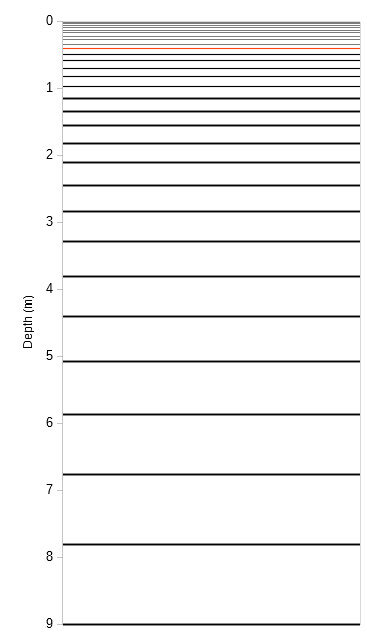
\includegraphics{profondef.png}
    \caption{Depth of each consecutive layer in the model, the tenth layer is marked in red.}
    \label{profondef}
\end{figure}{}

The convergence is guaranteed if time steps and space steps meet : \[\frac{k dt}{c\rho dz^2}<=0.25\]

At the bottom layer, we include areothermal energy coming from the core. Estimates range from 19 mW/m$^2$ to 30 mW/m$^2$, given the uncertainties and the challenges in observations.

    \subsection{implementation of slopes}
    When considering topography the energy balance is adapted by the following :
    \begin{itemize}
        \item incidence angle of solar light over the sloped terrain changes from $\cos{\zeta} $ to $$\cos{ \zeta_s} = \cos{ \alpha} \cos{ \zeta} - \sin{ \alpha} \sin{zeta}\cos{\Delta a}$$
        with $\Delta a$ the difference in azimuth between the gradient slope of angle $\alpha$ and the sun. 
        \item reevaluation of the atmospheric fluxes from sources on the field of view of the slope, i.e. a factor $\cos^2{\alpha/2}$ due to the reduced solid angle of atmosphere over the slope.  
        \item longwave emission due self-heating of the surrounding flat terrain 
       \[Q_{land} = \epsilon \sigma T_{land}^4\sin{\alpha/2}\]
    \end{itemize}{}

\section{Thermal properties}
    \subsection{}
    Inertia maps given by (Putzig 2007) are measures of thermal properties mapped over the surface of Mars. Taken from TES aboard the orbiter Mars Global Surveyor, it gives a large-scale distribution of thermal inertia. 
    Focusing over the regions we are interested in, namely the Newton Crater and the Gale Crater, we can take the thermal inertia to be 200-300 J m-2 K-1 s-1/2 or t.u.i. 
    Thermal inertia is given by $\sqrt{k\rho c}$ with conductivity and heat capacity. 
    \subsection{}
    Observation of thermal inertia doesn't allow distinguishing individual values of $k$, $\rho$ and $c$. The TCEP measurements made by Phoenix in 2008 gives individual values for $k$ and $c$. 
    The baseline value of $k$ given by TECP is $0.085$ WK-1m-1. 
    Having a fixed value of the volumetric heat capacity $\rho c$ at $1.05 10^6$ J m-3 K-1 , the range in thermal inertia for mid-latitudes yields a range in conductivity from $0.01$ WK-1m-1 (corresponding to 200 t.u.i) to $.15$ WK-1m-1 (corresponding to 400 t.u.i), spanning an order of magnitude.
    The increase of conductivity with respect to increasing temperature is explained by the heat capacity changes. It is due to phonons propagation and linked to the increase in their mean free path. 
    
    \subsection{}
    These measurements are based on surface and sub-surface measurement of regolith properties. InSight is a lander which one of the aims is measuring the behaviour of the regolith at depth. Results are expected to enrich the knowledge about depth temperature and properties, including the depth of the ice table and heat flow data. 

\section{Layers of the soil}
    \subsection{}
    Direct global measurement of the subsurface (deeper than the first centimetres) being not yet achieved, subsurface ice has been studied using diffusive models of H20 evolution in the long term and global scale. Here it is assumed that the subsurface ice is shallow at mid-latitudes, the icetable to be the order of tens of cm deep. The ice presence at the surface is thought to be deeper than two meters. 
    These are baseline numbers, as models are being formulated that suggest persistence of shallow ice in porous interstices, notably in equatorial regions.
    
    \subsection{}
    The thermal properties of an ice cemented soil are the combination of thermal properties of dry soil and ice, under the assumption that ice is distributed evenly in the soil following Schorghofer and Aaronson. 
    \[k = k_{soil} + \phi k_{ice}-\],
    and the same combination is done with $\rho c$, where $\phi = 0.4$ is the porosity, which stems from study of soil analogs. $f_i$ ice the ice-fraction of ice in the voids. In Martian thermal and pressure conditions, the ice I values for $k_{ice}=3.2WK-1m-1 $, $c_{ice} = 1540 J kg-1K-1$ $\rho _{ice}=927 kg m-3$ are taken.
    
\section{Brines}
    Brines are high-concentration solution of salt in water. The presence of perchlorates on the surface of Mars and particularly at locations to recurring slope lineae is documented. The most widely found cations are magnesium and sodium.
    Other salts have been observed (chlorates, chlorides, sulfates...)
    We will thus concentrate on these two salts. 
    The main purpose of the salts is lowering the fusion point of the water. It would allow subsurface ice to melt when the temperature is not low enough for pure water to melt. The phase diagrams for magnesium and sodium perchlorate are thus. 
    
    The eutectic composition is the concentration at which the fusion point is the lowest (eutectic temperature). This is for the specific concentration of 44wt\% for magnesium perchlorate, resulting in a temperature of 206 K, and 52wt\% for sodium perchlorates, yielding a fusion point at 236K. 
    The specific concentration of these salts in the water is not yet know, we will then consider a wide range of concentrations. The freezing temperatures with respect to the concentration are on the following table.
    
    \begin{center}

    \begin{tabular}{|c|c|c|c|}
    \hline
     Salt/concentration & 5 \% & 20 \% & 35 \%\\
     NaClO$_4$ & 272 K & 266 K & 257 K \\
     MgClO$_4$ & 270 K & 264 K & 243 K \\
    \hline
    \end{tabular}{}
    \end{center}

    
\chapter{Results}
To understand the role of the slope orientation and steepness, figure \ref{fig:tvslopenewton} shows the annual average maximum and minimum temperature at the latitudes of two craters, Gale crater (-5), and Newton crater (-41), where RSLs were documented, for a continuous range of slopes.
Positive slope index is a slope facing the equator and negative slope is a pole-facing gradient.
The plot validates the model as it replicates successfully the graph from Chevrier (2012). \\
\begin{figure}
    \centering
    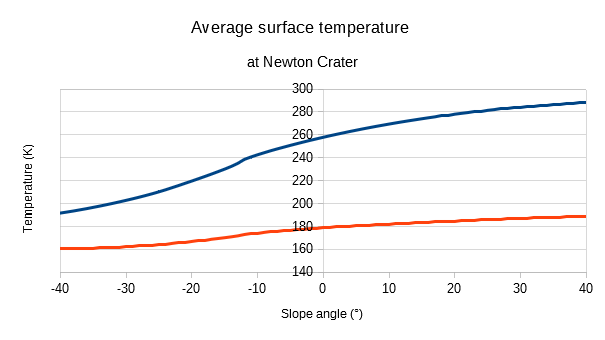
\includegraphics[width=.9\textwidth]{graphs/0108-newton-tvslope.png}
    \caption{Average maximum (red line) and average minimum (blue line) surface temperatures at the latitude of Newton Crater by slope.}
    \label{fig:tvslopenewton}
\end{figure}{}

If the presence of dry ice is implemented in the thermal model, the frozen ground has a temperature of 148 K. This type of ice can appear on slope that are facing the poles on slopes over 11 degrees. The ice remains present over a period of several days around the local winter solstice. This causes the apparent discontinuity that can be seen on figure \ref{fig:tvslopenewton}. 

Temperatures on the slopes around the equator are much more stable (figure \ref{tvslopegale}) and have a maximum around a 12 degrees equator facing slope.\\ 

\begin{figure}
    \centering
    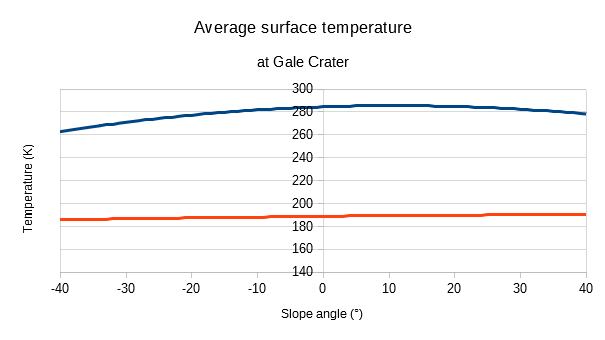
\includegraphics[width=.9\textwidth]{graphs/0108-gale-tvslope.png}
    \caption{Average maximum (red line) and average minimum (blue line) surface temperatures at the latitude of Gale Crater (near the equator) by slope.}
    \label{tvslopegale}
\end{figure}{}

Maximum, minimum and daily average temperatures on a flat terrain are compared with sloped surfaces. The slope steepness will be hereafter 35 degrees for the Newton Crater and 15 degrees for the Gale crater.  \\
\begin{figure}
    \centering
    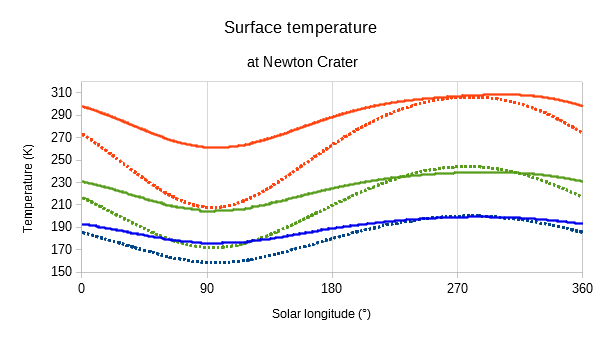
\includegraphics[width=.9\textwidth]{graphs/0108-newton-tempannu-flat.png}
    \caption{Maximum (red line), minimum (blue line), daily average (green line) surface temperatures for a flat terrain (dashed lines) and 35 \degree slope facing the equator (solid line)}
    \label{tempannunewton}
\end{figure}{}

Temperature on the slopes are generally higher than on a flat soil (figure \ref{tempannunewton}) on Newton crater, on a equator facing slope, with a lower seasonal variability. The local summer is at 270\degree of solar longitude. Nighttime temperatures all year round are around 190 K due to the relatively low thermal inertia and absence of a strong atmosphere. \\

\begin{figure}
    \centering
    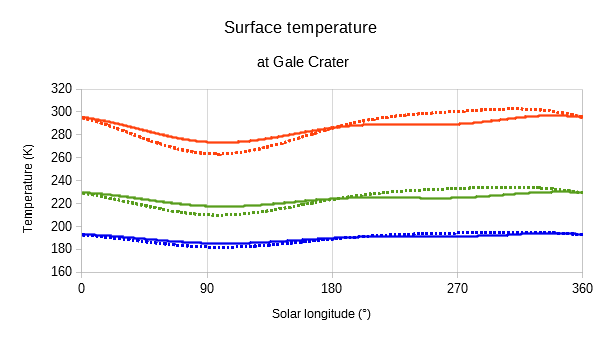
\includegraphics[width=.9\textwidth]{graphs/0108-gale-tempannu-flat.png}
    \caption{Maximum (red line), minimum (blue line), daily average (green line) surface temperatures for a flat terrain (dashed lines) and 15 \degree slope facing the equator (solid line)}
    \label{tempannugale}
\end{figure}{}
The low latitude lead to weaker seasonal variations (figure \ref{tempannugale}), where the same smoothing effect of the slope is observed. Note that the slope is much lower than figure \ref{tempannunewton}. \\

When the sun is up, more than 90 \% of the incoming energy comes from sunlight (figure \ref{qpropnewton}), and a negligible fraction spans from surrounding land and the atmosphere. The contribution resulting from heating of the atmosphere is considered constant during all martian day (as in Schorghofer) and is the leading nighttime term. The land contribution contributes up to 40 \% contribution to the heat flux just after sunset. As this radiative flux contribution linked to the temperature of the surface, it peaks at noon and is minimal just before sunrise (figure \ref{qnewton}. \\

\begin{figure}
    \centering
    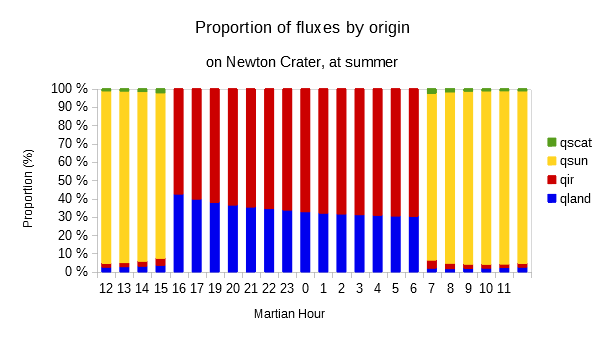
\includegraphics[width=.9\textwidth]{graphs/0108-newton-q-prop.png}
    \caption{Proportion of fluxes}
    \label{qpropnewton}
\end{figure}{}
\begin{figure}
    \centering
    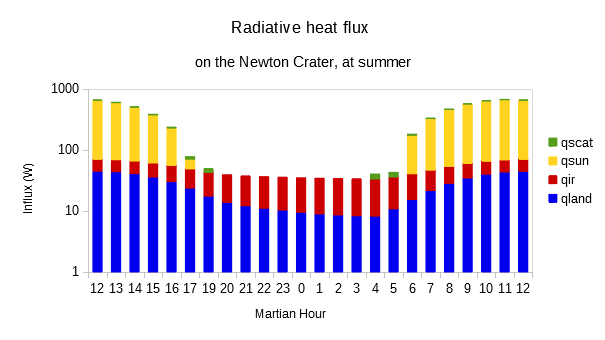
\includegraphics[width=.9\textwidth]{graphs/0108-newton-q.png}
    \caption{Incoming fluxes (log scale), in summer, on Newter Crater}
    \label{qnewton}
\end{figure}{}

As the conductivity can span over an order of magnitude, the influence of such changes determine the sensitivity of the model to this input variable (figure \ref{diffknewton}). The values are 0.015WK-1m-1 for the dashed lines, 0.15WK-1m-1  for the dotted lines, and 0.085WK-1m-1 for solid lines. The most important difference is a lower overall minimum temperature for a low thermal conductivity. \\

\begin{figure}
    \centering
    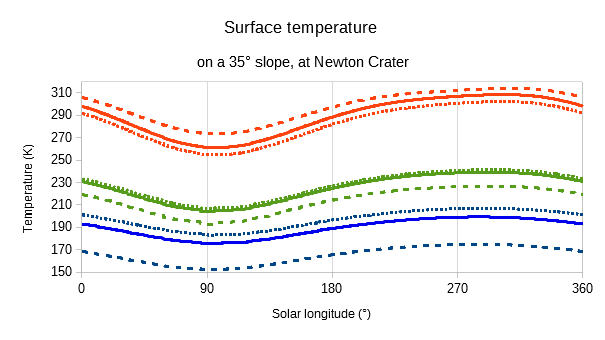
\includegraphics[width=0.9\textwidth]{graphs/0108-newton-diffk.png}
    \caption{Maximum (red line), minimum (blue line), daily average (green line) surface temperatures for different values of thermal conductivity}
    \label{diffknewton}
\end{figure}{}

The temperature evolves through the martian day heavily, from 200 K to 310 K on the warmest day of the year (figure \ref{hourlynewton}). Midday is the hottest hour of the day, with temperature slightly decreasing through the afternoon and night, reaching a minimum before sunrise. On the coldest day, the same trend is followed though the temperatures are much lower (40 K difference at the most). \\
\begin{figure}
    \centering
    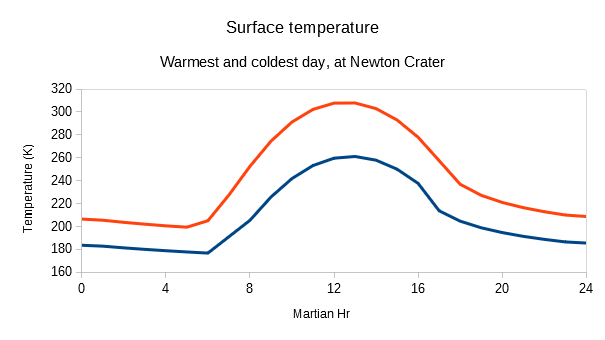
\includegraphics[width=0.9\textwidth]{graphs/0108-newton-hourly.png}
    \caption{Surface temperature on the warmest day (red) and coldest (blue) day of the year, on a 35 \degree slope}
    \label{hourlynewton}
\end{figure}{}

Near the equator, seasonal variations are much lower (figure \ref{hourlygale}), with a maximal temperature difference not exceeding 20 K. \\
\begin{figure}
    \centering
    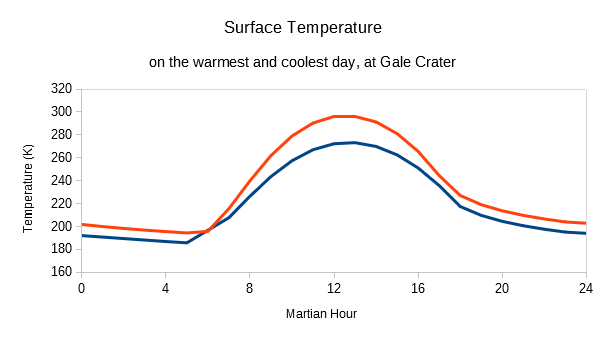
\includegraphics[width=0.9\textwidth]{graphs/0108-gale-hourly.png}
    \caption{Surface temperature on the warmest day (red) and coldest (blue) day of the year, on a 15 \degree slope}
    \label{hourlygale}
\end{figure}{}

In-depth modelled temperature based on constant thermal properties are sustained after sunset in summer (figure \ref{profilenewton}), at 10 cm deep being over 240 K for 12 martian hours straight.  
\begin{figure}
    \centering
    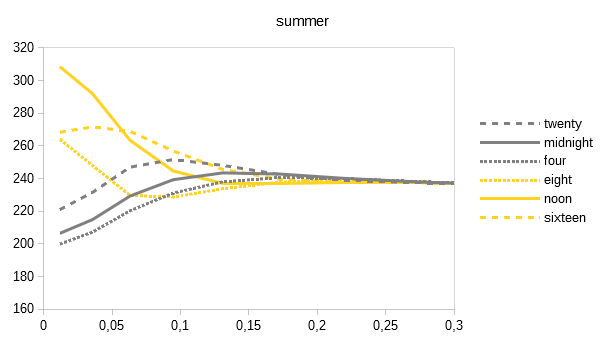
\includegraphics[width=0.5\textwidth]{graphs/0208-newton-profile-summer.png}
    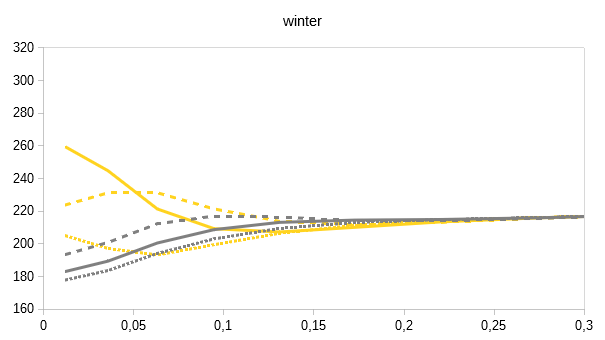
\includegraphics[width=0.5\textwidth]{graphs/0208-newton-profile-winter.png}
    \caption{Caption}
    \label{profilenewton}
\end{figure}{}

Modelling a temperature-dependant conductivity or a conductivity rising with depth. \\

\chapter{Discussion}

\section*{Conclusion}

\printbibliography 

\end{document}
